\documentclass[letterpaper, 10 pt, conference]{ieeeconf}  % Comment this line out if you need a4paper
%\documentclass[a4paper, 10pt, conference]{ieeeconf}      % Use this line for a4 paper
\IEEEoverridecommandlockouts                              % This command is only needed if 
                                                          % you want to use the \thanks command
\overrideIEEEmargins                                      % Needed to meet printer requirements.

\title{\LARGE \bf
  Longitudinal Trajectory Planning and Tracking for Fixed-Path Autonomous Driving
}

\author{
  Robert G. Cofield $^{1}$,
  Rakesh Gupta $^{2}$,
  Ambarish Goswami $^{3}$,
  and
  David Bevly $^{4}$
  \thanks{
    * This work is supported by Honda Research Institute USA.
  }
  \thanks{
    $^{1}$ Robert G. Cofield is a graduate researcher at Auburn University's GPS \& Vehicle Dynamics Laboratory.
  }
  \thanks{
    $^{2}$ Rakesh Gupta ...
  }
  \thanks{
    $^{3}$ Ambarish Goswami ... 
  }
  \thanks{
    $^{4}$ David Bevly ...
  }
}

\usepackage[pdftex]{graphicx}
\usepackage[hypcap]{caption}


%%%%%%%%%%%%%%%%%%%%%%%%%%%%%%%%%%%%%%%%%%%%%%%%%%%%%%%%%%%%%%%%%%%%%%%%%%%%%%%%
%%%%%%%%%%%%%%%%%%%%%%%%%%%%%%%%%%%%%%%%%%%%%%%%%%%%%%%%%%%%%%%%%%%%%%%%%%%%%%%%
%%%%%%%%%%%%%%%%%%%%%%%%%%%%%%%%%%%%%%%%%%%%%%%%%%%%%%%%%%%%%%%%%%%%%%%%%%%%%%%%

\begin{document}

\maketitle
\thispagestyle{empty}
\pagestyle{empty}

%%%%%%%%%%%%%%%%%%%%%%%%%%%%%%%%%%%%%%%%%%%%%%%%%%%%%%%%%%%%%%%%%%%%%%%%%%%%%%%%
\begin{abstract}

When planning trajectories for an autonomous ground vehicle operating on roadways, it is common to employ the path-velocity decomposition (i.e., path planning is performed prior to planning the speed that the vehicle will take along the chosen path).
Given a desired path, we present a novel method of planning longitudinal trajectories (i.e., the time derivatives of position in the body-forward direction) along that path.
This method first segments the path using an arbitrary set of kinematic or dynamic constaints which may be functions of the desired path.
Each segement is then planned sequentially by choosing a piecewise constant jerk profile.
The jerk profile is intelligently chosen from a set of pre-solved profiles such that acceleration is continuous throughout the entire path.
The resultant trajectory plan can then be easily sampled to provide a reference for real-time vehicle control.
This method is shown to be efficient and reliable for use in online planning with a test vehicle.

\end{abstract}
%%%%%%%%%%%%%%%%%%%%%%%%%%%%%%%%%%%%%%%%%%%%%%%%%%%%%%%%%%%%%%%%%%%%%%%%%%%%%%%%

%%%%%%%%%%%%%%%%%%%%%%%%%%%%%%%%%%%%%%%%%%%%%%%%%%%%%%%%%%%%%%%%%%%%%%%%%%%%%%%%
\section{Introduction}
\label{sec:introduction}

... autonomous vehicles ... \emph{The 1st sentence is the hardest}.
One such task is computing a tentative reference trajectory plan for travelling from one point to another.
While the set of possible paths between any two points is infinite, it is typically heavily restricted by consideration of constraints such as traversability and legally available travel lanes, among others.
The intended speed, acceleration, and higher derivates of position with respect to time are also subject to constraints.
These may include legal speed limits, engine dynamics, desired sideslip limits, traction availability, and rollover concerns.

% intersection of path-planning constraints and speed-planning constraints is vehicle dynamics

% review of literature for a few paragraphs]
%  - searching planners (OMPL stuff)
%  - robot joint planning --> constant jerk intervals

% We will use the path-velocity decomposition
% mention using curvilinear CS
% 

% tracking
Once a trajectory plan is formulated, it must be utilized online in order for a reference signal to be sent to the controllers which govern steering, braking, and engine speed.
This is the trajectory tracking problem, which is discussed in Section \ref{sec:trajectorytracking}.

% mention using same cuvilinear cs scheme to project onto path

\section{Trajectory Planning}
\label{sec:trajectoryplanning}

For the purposes of this work, the objective of trajectory planning is to take a 2 dimensional (horizontal plane) path, and compute a series of constant jerk intervals for motion along the length of the path which is time optimal yet still falls within constraints on speed, acceleration, and jerk.
It is assumed that an independent path planner will produce this information.
Prescribed initial and end conditions for position, speed, and acceleration must also be honored. 
This means that the desired trajectory plan is one dimensional, so using curvilinear coordinates will significantly simplify the solution.

% Need some lead in here?

% \subsection{Simple Case}

Consider, as a starting point, the case in which a vehicle is at rest and needs to accelerate to some travelling speed, maintain that speed for some distance, then brake to a stop at a prescribed end location.
Figure \ref{fig:7phaseprofile} shows this trajectory over time.
The problem is defined by the vector of known values $\bf{G} = [v_i, v_f, L, v_m]$, being initial speed, final speed, the total distance, and the speed limit, respectively.
If the desired peak acceleration and jerk ($a_m$ and $j_m$, respectively) are known, then the profile with $M$ jerk phases (7 in this case) can be generated by solving for the time intervals $[\Delta t_1, \Delta t_2, ..., \Delta t_M]$.
Jerk and peak acceleration may be different when reducing speed versus increasing speed to more closely mirror human driving behavior \emph{Citation}.
The user-defined parameters now become $\bar{a}_m = [a^+_m , a^-_m]$ and $\bar{j}_m = [j^+_m , j^-_m]$.
There are, however multiple solutions for $\Delta t_2$, $\Delta t_4$, and $\Delta t_6$.
The proper solution must be chosen by eliminating negative and complex solutions.

\begin{figure}[thpb]
  \centering
  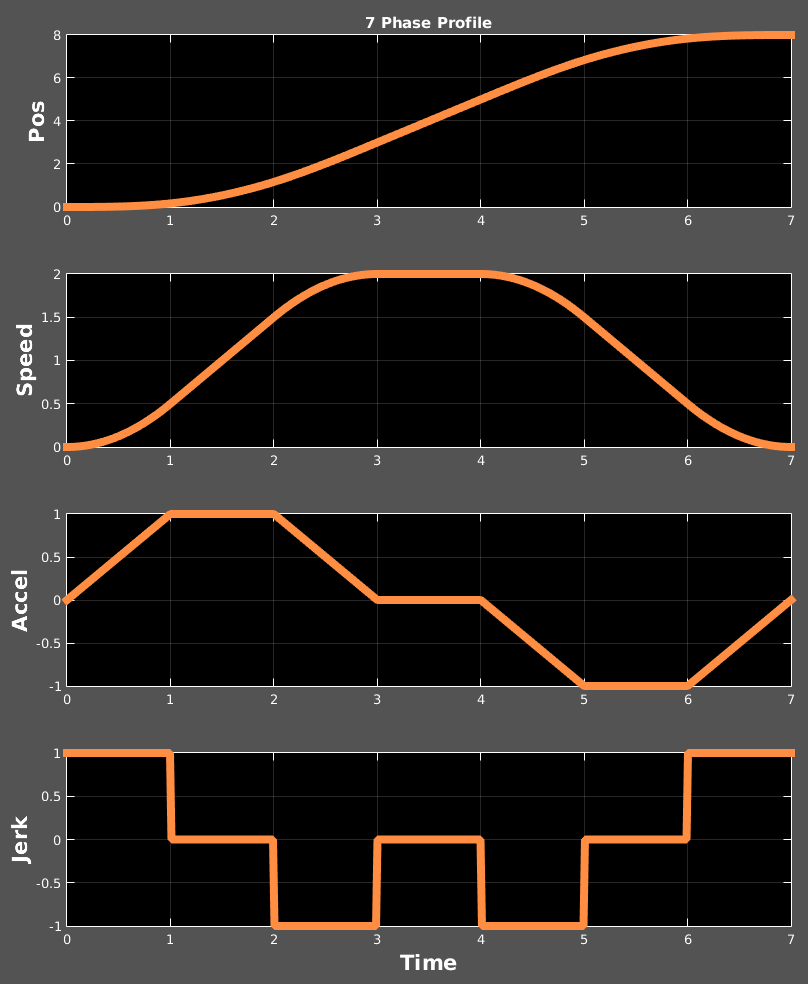
\includegraphics[width=1.0\columnwidth]{graphics/7phaseprofile.png}
  \caption{7 phase constant jerk profile along curvilinear distance axis.}
  \label{fig:7phaseprofile}
\end{figure}

It is obvious that there are many cases in which this solution will fail.
For instance, if $L$ is sufficiently short and $v_m$ is sufficiently high, then it will not be possible to ever reach $v_m$ with realistic values of $\bar{a}_m$ and $\bar{j}_m$.
The authors then propose that 4 other basic profiles be defined, and an algorithm constructed which judiciously chooses the appropriate profile for every segment defined by a vector $\bf{G}$.
The other profiles are explained below in section \ref{sec:jerkprofiles}.
A path is then a set of $i$ segments, each of which is defined by a set of parameters $G_i$ and can be solved indivually in sequence.
Determination of where to break a path into segments is discussed below in Section \ref{sec:pathsegmentation}.

\subsection{Jerk Profiles}
\label{sec:jerkprofiles}

asdf

\subsection{Path Segmentation}
\label{sec:pathsegmentation}

asdf

\section{Trajectory Tracking}
\label{sec:trajectorytracking}

asdf


%%%%%%%%%%%%%%%%%%%%%%%%%%%%%%%%%%%%%%%%%%%%%%%%%%%%%%%%%%%%%%%%%%%%%%%%%%%%%%%%



\end{document}